\documentclass[11pt, oneside]{article}
\usepackage[bottom=2.5cm,top=2.5cm]{geometry}
\geometry{a4paper}
\usepackage{graphicx}
\usepackage{amssymb}
\usepackage[utf8]{inputenc}
\usepackage[brazil]{babel}
\usepackage{color}
\usepackage{float}
\usepackage{hyperref}
\bibliographystyle{apalike}
\usepackage{indentfirst}

\title{Briefing Space Weather}
\date{2022/04/25}

\begin{document}
\maketitle 

 \section{Imageador All-Sky} 
 \subsection{Responsável: LUME} 
 
\begin{figure}[H]
    
                        \centering
   
                             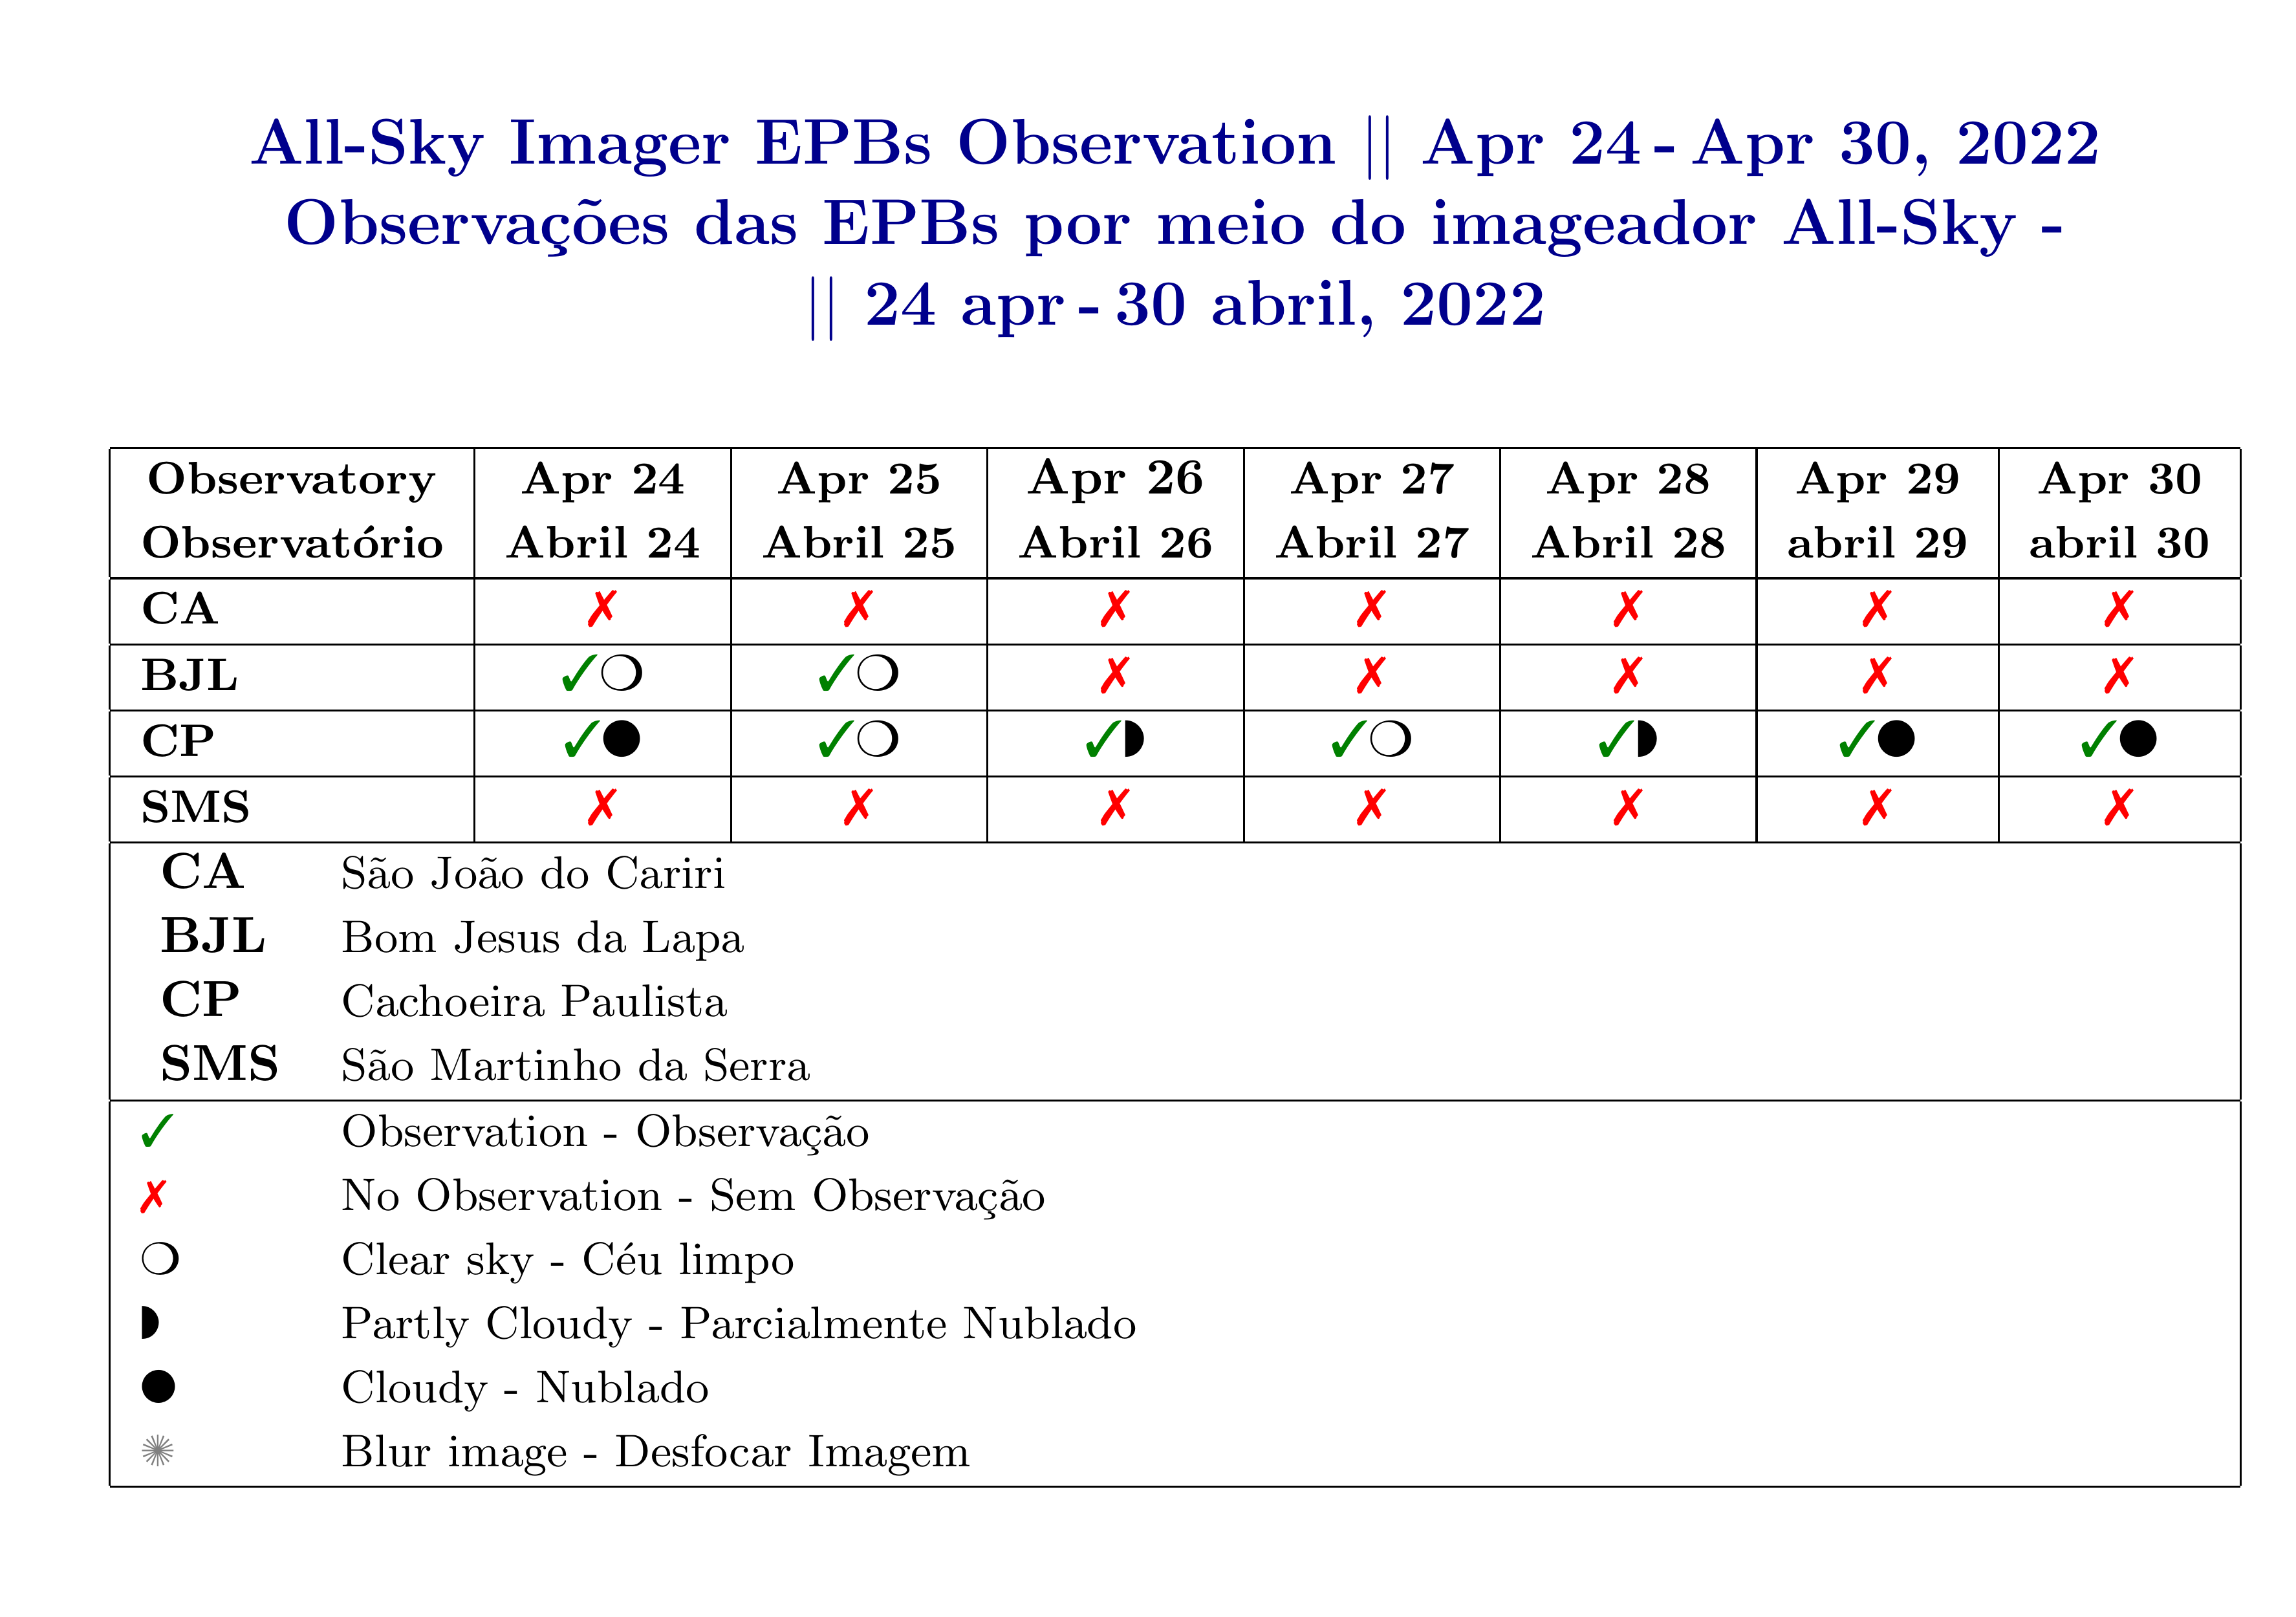
\includegraphics[width=14cm]{./figures//figureImager_0.png}

                        \end{figure}

                     \begin{itemize} 
 \item  No observatorio de Sao Joao do Cariri, nao houve obvervacao todo semana e nao foi observado bolhas. 
\item  No observatorio de Bom de Jesus da Lapa, entre os dias 26 de bril e 30 de abril, nao houve observacao. Todo semana, nao observa bolhas. 
\item  No observatorio de Cachoeira Paulista, nao foi observado bolhas de plasma durante o perıodo. Os dias 24, 29 e 30 de abril, ceu estava nublado. 
\item  Por fim, no observatorio de Sao Martinho da Serra, nao observa bolhas durante semana. 
\end{itemize} 
 TEC 
\begin{itemize} 
 \item  Foi observado bolhas de plasma durante todo o perıodo especificamente no dias que tem mapa de TEC cobrindo o Brasil. No entanto, como a sazonali- dade de bolhas esta no fim, as bolhas apresenta dimensoes espaciais pequenas e fica difıcil de observar no mapas de TEC. 
\end{itemize} 
 

\end{document}